%%%%%%%% InferCell paper 1: ICML 2026 two-column format, [preprint] mode %%%%%%%%
% Journal-agnostic draft (target: Cell Systems or PLOS Computational Biology).
% Build: latexmk -pdf main.tex

\documentclass{article}

\usepackage{microtype}
\usepackage{graphicx}
\graphicspath{{figures/}}
\usepackage{booktabs}
\usepackage{nicefrac}
\usepackage{hyperref}
\newcommand{\theHalgorithm}{\arabic{algorithm}}

% [preprint] shows authors and drops the review-mode footer.
\usepackage[preprint]{icml2026}

\usepackage{amsmath}
\usepackage{amssymb}
\usepackage{amsfonts}
\usepackage{mathtools}
\usepackage{xcolor}
\usepackage[capitalize,noabbrev]{cleveref}

\hypersetup{
    hidelinks,
    colorlinks = true,
    citecolor  = cyan,
    urlcolor   = black,
    linkcolor  = magenta,
    pdftitle   = {InferCell: inference-first whole-cell modelling},
    pdfauthor  = {Tom Kimpson},
}

% Placeholders. Red text marks anything that is not yet a result or a decision.
% grep for \placeholder before any submission; check-arxiv-llm-compliance flags leftovers.
\newcommand{\placeholder}[1]{\textcolor{red}{[#1]}}

% \placeholderfig{width}{height}{text}: a framed box that stands in for a figure.
\newcommand{\placeholderfig}[3]{%
  \fbox{\parbox[c][#2][c]{#1}{\centering\textcolor{red}{\small #3}}}}

% Names used often.
\newcommand{\IC}{\textsc{InferCell}}
\newcommand{\syn}{JCVI-syn3A}
\newcommand{\Mzero}{M0}
\newcommand{\Rhat}{\widehat{R}}
\newcommand{\sigb}{\sigma_{\mathrm{b}}}
\newcommand{\code}[1]{\texttt{#1}}

%% Every number quoted in the text, with its source. Use \pn{key}.
%% Typed by hand from the result files named on each line (no generator yet).
%% An undefined key stops the build.
\makeatletter
\DeclareRobustCommand{\pn}[1]{\@ifundefined{pn@#1}{\PackageError{numbers}{Undefined paper number `#1'}{Add it to numbers.tex.}\textbf{??}}{\@nameuse{pn@#1}}}
\providecommand{\pndef}[2]{\@namedef{pn@#1}{#2}}
\makeatother

%% --- The reduced syn3A model --------------------------------------------
\pndef{model.rxn}{22}% spec/spec.md §2 table; docs/src/user-guide/reduced-syn3a.md
\pndef{model.odemodules}{four}% spec/spec.md §0
\pndef{model.genes}{17}% spec/spec.md §0
\pndef{model.jumpmodules}{three}% spec/spec.md §0
\pndef{model.jumprxn}{52}% src/organisms/coreA (agent survey of the registry)
\pndef{model.species}{32}% COREA_SPECIES dynamic species, src/organisms/coreA/registry.jl
\pndef{model.chemostats}{5}% COREA_SPECIES chemostats
\pndef{model.removed}{92\%}% spec/spec.md §0
\pndef{model.cycle}{6{,}300}% COREA_CYCLE_S, seconds
\pndef{model.cyclewall}{32.2}% spec task 13.7, job 17298242 (s per cycle, warm)
\pndef{model.handshake}{5.11}% spec task 13.7 (ms per handshake)

%% --- Framework -------------------------------------------------------------
\pndef{fw.edgekinds}{seven}% src/edges.jl EDGE_KINDS
\pndef{fw.redcats}{16}% src/labels.jl REDUCTION_CATEGORIES
\pndef{fw.tests}{28{,}709}% docs/handoff.md, suite job 19042448 at 67c9eef

%% --- M0 ---------------------------------------------------------------------
\pndef{mzero.cells}{50}% spec/phases/16-recovery.md D16.4
\pndef{mzero.horizon}{600}% M0_HORIZON_S, src/organisms/coreA/m0.jl
\pndef{mzero.npar}{six}% M0_TARGETS (5) + sigma_b

%% --- Gains (F1) -----------------------------------------------------------
\pndef{gain.txlo}{0.044}% spec/spec.md ~L3093 (0.043742)
\pndef{gain.txhi}{0.051}% spec/spec.md ~L3093 (0.050579)
\pndef{gain.gtplo}{0.008}% spec/spec.md ~L3093 (0.0078915)
\pndef{gain.gtphi}{0.012}% spec/spec.md ~L3093 (0.0117062)
\pndef{gain.tl}{0.091}% dev/scripts/translation_diagnostics_result.md (median 0.0910)
\pndef{gain.kd}{0.1}% RNAPOL_KD, mM, src/organisms/coreA/transcription.jl:50
\pndef{gain.atp}{3.65}% ATP, mM, discussion note §6

%% --- Information bounds (track A) ----------------------------------------
\pndef{info.mzeroptsg}{0.47}% dev/scripts/sensitivity_88_m0_result.md
\pndef{info.mzerobracket}{0.68}% same
\pndef{info.ptsg}{0.10}% dev/scripts/sensitivity_88_corea_result.md, C=200, sigma_b 10%
\pndef{info.ptsgbracket}{0.19}% same
\pndef{info.eno}{0.13}% same
\pndef{info.enobracket}{0.75}% same
\pndef{info.enotx}{0.999}% spec/spec.md §1 (ENO under transcripts only)
\pndef{info.Rmzero}{64}% sensitivity_88_m0_result.md, sigma_b 10%
\pndef{info.Rcorea}{70}% sensitivity_88_corea_result.md, C=200, sigma_b 10%

%% --- V6, V7, F10 (the exact reference) -------------------------------------
\pndef{vsix.chains}{4}% dev/scripts/v6_16a9b_result.md
\pndef{vsix.sweeps}{1{,}650}% same
\pndef{vsix.rhat}{1.007}% same
\pndef{vsix.ess}{1{,}081}% same (bulk)
\pndef{vsix.cpuh}{6{,}810}% same (6,809.7)
\pndef{vseven.R}{50}% dev/scripts/v7_16a9b_result.md
\pndef{vseven.maxdev}{0.164}% same (krnadeg)
\pndef{vseven.band}{0.244}% same
\pndef{vseven.cov}{29 of 30}% spec/phases/16-recovery.md §12 2026-10-22
\pndef{vseven.lowess}{23}% replicates with min bulk ESS < 100
\pndef{vseven.cpuh}{33{,}900}% v7_16a9b_result.md
\pndef{ften.cpuh}{507.5}% dev/scripts/f10_16a10_result.md
\pndef{ften.dmean}{0.12}% same, max |Δmean|/SD_ref
\pndef{ften.sdlo}{0.91}% same
\pndef{ften.sdhi}{1.19}% same
\pndef{ften.fbamargin}{0.020}% same
\pndef{ften.speedup}{13}% 6,810 / 507.5
\pndef{cost.fullscale}{21{,}000}% spec/phases/16-recovery.md §12 2026-10-22 (projected)
\pndef{cost.kone}{1{,}000}% spec §8 K1 bound, CPU-h per posterior

%% --- Track B: the formalism swap --------------------------------------------
\pndef{jg.gtplo}{10}% dev/scripts/jensen_rethink_89_result.md (% GTP below)
\pndef{jg.gtphi}{16}% same
\pndef{jg.deltain}{26 of 28}% same (δ inside KG's null)
\pndef{jg.mfin}{5 of 28}% same (uncorrected)
\pndef{jg.kgnulllo}{36}% same (% a right description passes KG)
\pndef{jg.kgnullhi}{56}% same
\pndef{jg.biaslo}{2.4}% dev/scripts/jensen_bias_89_result.md (krnadeg, posterior SD)
\pndef{jg.biashi}{3.1}% same
\pndef{jg.cpuh}{48}% jensen_rethink_89_result.md
\pndef{rii.maxdelta}{0.0122}% dev/scripts/route_ii_89_result.md
\pndef{rii.mzero}{1.1}% docs/handoff.md (s per M0 600 s solve)
\pndef{rii.corealo}{9}% docs/handoff.md (s per 6,300 s solve)
\pndef{rii.coreahi}{12}% same


\icmltitlerunning{InferCell: inference-first whole-cell modelling}

\begin{document}

\twocolumn[
  \icmltitle{InferCell: inference-first whole-cell modelling}

  \begin{icmlauthorlist}
    \icmlauthor{Tom Kimpson}{aff1}
    \icmlauthor{\placeholder{Co-authors}}{aff1}
  \end{icmlauthorlist}

  \icmlaffiliation{aff1}{\placeholder{Affiliations}}

  \icmlcorrespondingauthor{Tom Kimpson}{\placeholder{email}}

  \icmlkeywords{whole-cell modelling, Bayesian inference, uncertainty quantification,
    hybrid stochastic models, simulation-based calibration, JCVI-syn3A}

  \vskip 0.3in
]

\printAffiliationsAndNotice{}

\begin{abstract}
Whole-cell models simulate a living cell from its molecular parts. They fix every
parameter to one value, so each prediction is a single sample with no error bar.
The models cannot say how much of a prediction the data support. Inference is hard
because the models mix deterministic and stochastic formalisms, the stochastic paths
are latent, and no parameter is shared across the boundary between the two blocks.
We present \IC{}, a Julia framework that makes inference a
first-class operation in whole-cell modelling. Every parameter is a prior
distribution with a recorded source. Modules couple through typed edges, and the
framework checks the composition and lists every reduction from the published model.
The framework can run the same gene-expression interface as an exact stochastic
process or as a mean-field ODE, so the whole cell compiles to one differentiable ODE
for gradient-based inference, at a declared and measured cost. We test the framework on a reduced model of the minimal cell
\syn{}, with four ODE modules and three stochastic modules. An exact sampler passes
simulation-based calibration on a two-gene reference system over \pn{vseven.R}
replicate datasets. \placeholder{Approximate method result (B7): agreement with the
exact posterior on M0, cost ratio.} \placeholder{Full-scale result (B8): calibration
on the reduced syn3A model; metabolite data shrink a gene-expression parameter they
do not measure.} \placeholder{Uncertainty-budget sentence: x\% of the uncertainty in
a prediction comes from parameters that no measurement supports.}
\end{abstract}

\placeholder{Author summary (PLOS CB, $\le$ 200 words) or Highlights and eTOC blurb
(Cell Systems): write once the venue is chosen.}

\section{Introduction}
\label{sec:intro}

A whole-cell model simulates a cell from its molecular parts. The first such model
described \textit{Mycoplasma genitalium} with \pn{lit.karrsub} coupled submodels
\citep{karr2012whole}. Later models covered \textit{Escherichia coli}
\citep{macklin2020simultaneous} and the minimal cell \syn{}, first well stirred
\citep{thornburg2022fundamental} and then in space and time over a full cell cycle
\citep{thornburg2026bringing}. Each one joins
metabolism, gene expression, growth and division in one simulation, and each
reproduces measured behaviour of a real cell.

All of these models are forward simulators. Each one takes hundreds or thousands of kinetic
parameters from the literature, sets each to one value, and integrates forward in
time. The output is one trajectory. That trajectory is one sample from the
distribution of trajectories that the parameter knowledge allows. The model does not
know the width of that distribution. When a model predicts a doubling time, a reader
cannot tell whether the prediction holds for every plausible parameter set or depends
on a few uncertain values.

The missing error bar is a gap in the scientific reasoning. Every parameter in a
whole-cell model is uncertain. A rate measured in one organism, at one temperature,
in one medium, is then used in another organism under other conditions. The
uncertainty is real, and it propagates through coupled nonlinear dynamics into every
prediction. A framework that stores each parameter as a single number has no place
to put this uncertainty. It cannot ask how uncertain a prediction is, and it cannot
ask which data would reduce that uncertainty.

\subsection{Why whole-cell models do not do inference}

Bayesian inference answers both questions. It treats each parameter as a
distribution, updates the distribution with data, and propagates the result into
predictions. Systems biology argued for this approach long ago
\citep{babtie2017how}. Whole-cell models still do not use it, for the
following reasons.

\begin{enumerate}
  \item \emph{No place for uncertainty.} The frameworks store parameters as
  floating-point values in a dictionary. The source of each value is in a
  spreadsheet or a supplement, not in the model. When two sources disagree, the code
  picks one without a record.
  \item \emph{Mixed formalisms.} Metabolism is a set of ordinary differential
  equations (ODEs). Gene expression is a stochastic jump process. The two exchange
  state on a fixed clock. No single likelihood and no standard sampler covers both.
  \item \emph{Latent paths.} The stochastic block has a hidden path: the exact
  times of each transcription and translation event. The likelihood of the data
  integrates over all such paths, and that integral has no closed form.
  \item \emph{Cost.} Inference needs many simulations. For a whole-cell model the
  number of simulations, not the cost of one, sets the budget.
  \item \emph{No shared parameters.} In the published \syn{} model, no rate
  constant appears in both blocks. The blocks couple only through state. The
  standard methods for modular inference pass information through shared
  parameters \citep{plummer2015cuts,jacob2017better,carmona2020semimodular}.
  Here they have nothing to pass.
\end{enumerate}

\Cref{tab:frameworks} compares current whole-cell frameworks on these points.
Thornburg and coworkers balanced the metabolic parameters of \syn{} against each
other with a Bayesian method \citep{thornburg2022fundamental}. That step used
literature values for metabolism only. It did not infer parameters from dynamic
data through the coupled model.

\begin{table*}[t]
\caption{Capabilities of whole-cell modelling frameworks. A tick means that the
framework does this as part of its design. \placeholder{Every cell to be checked
against each framework's code and papers before submission.}}
\label{tab:frameworks}
\centering
\small
\begin{tabular}{@{}lcccc@{}}
\toprule
& Priors & Provenance & Inference & Declared \\
& & in model & on dynamics & reductions \\
\midrule
\textit{M.\ genitalium} \citep{karr2012whole} & \placeholder{?} & \placeholder{?} & \placeholder{?} & \placeholder{?} \\
\textit{E.\ coli} \citep{macklin2020simultaneous} & \placeholder{?} & \placeholder{?} & \placeholder{?} & \placeholder{?} \\
Vivarium \citep{agmon2022vivarium} & \placeholder{?} & \placeholder{?} & \placeholder{?} & \placeholder{?} \\
\syn{} \citep{thornburg2022fundamental,thornburg2026bringing} & \placeholder{?} & \placeholder{?} & \placeholder{?} & \placeholder{?} \\
\IC{} (this work) & \checkmark & \checkmark & \checkmark & \checkmark \\
\bottomrule
\end{tabular}
\end{table*}

\subsection{This work}

We present \IC{}, a framework that puts inference first. We do not claim that full
Bayesian inference over every parameter of a whole-cell model is possible today. We
claim that the framework must support inference as a basic operation, so that a
modeller can apply it where the data and the budget allow. Our contributions are:

\begin{enumerate}
  \item \textbf{A design for inference-first composition} (\cref{sec:design}). Every
  parameter is a prior with a recorded source. Modules couple through
  \pn{fw.edgekinds} kinds of typed edge. The framework checks that a composition is
  complete before it runs, and it lists every departure from the published model.
  \item \textbf{One interface with two descriptions} (\cref{sec:design}). The same
  gene-expression modules run as an exact stochastic process or as mean-field ODEs.
  In the second form the whole cell compiles to one ODE problem that automatic
  differentiation can pass through.
  \item \textbf{A reduced model of \syn{} with a real boundary} (\cref{sec:model}).
  It keeps \pn{model.rxn} metabolic reactions and \pn{model.genes} genes from the
  published model, and it keeps the two-way coupling between them.
  \item \textbf{A map of how information crosses the boundary}
  (\cref{sec:seam}), and calibrated inference across it (\cref{sec:results}). An
  exact sampler gives a calibrated reference. \placeholder{An approximate method
  agrees with it at a fraction of the cost, and scales to the full reduced model.}
\end{enumerate}

\placeholder{Last paragraph: a one-sentence statement of the main result, written
after B7 and B8.}

\section{InferCell: an inference-first design}
\label{sec:design}

\IC{} is written in Julia \citep{bezanson2017julia}. It uses the SciML solvers for
ODEs and jump processes \citep{rackauckas2017differentialequations}. This section
gives the design ideas. The documentation gives the full interface
(\cref{sec:availability}). \Cref{fig:architecture} shows the parts and how they
connect.

\begin{figure*}[t]
\centering
\placeholderfig{0.9\textwidth}{6cm}{Figure 1 (F11): the architecture. Parameters
with provenance feed modules; modules declare formalism and edges; the resolver
checks the composition; the composed model runs as the exact hybrid or as one
mean-field ODE; inference routines attach to each data stream. To be drawn.}
\caption{\textbf{The \IC{} architecture.} \placeholder{Caption to be written with the
figure.}}
\label{fig:architecture}
\end{figure*}

\subsection{Parameters are distributions with a source}

Each parameter in \IC{} is an object that holds a value, a prior distribution, a
role and a record of its source. The record names the file, the table and the
identifier the value came from, and the values that other files give for the same
identifier. Each parameter also has one of four labels for how well its prior is
informed:
\begin{itemize}
  \item \emph{balanced}: the value and width come from a balanced parameter table;
  \item \emph{prior default}: the source gives no width, so the prior is wide;
  \item \emph{asserted}: the source gives no uncertainty, so we set the prior;
  \item \emph{not imported}: the parameter is not in the source.
\end{itemize}
The loader does not choose silently between two files that disagree. It stops and
asks for a decision, and the decision is then part of the record. A user can ask
the composed model which priors no measurement supports. That question has a
direct answer, because the answer is in the model and not in a supplement.

\subsection{Modules couple through typed edges}

A module declares its states, its parameters and its formalism: ODE or jump. It
also declares how it touches the rest of the cell. \IC{} has \pn{fw.edgekinds} kinds
of coupling edge (\cref{tab:edges}). Each kind says what crosses the edge and on
which clock. Mass and currency edges act inside the ODE solve. Catalytic edges
and deferred costs cross every second, at the handshake between the two blocks.
Rate-constant edges cross every minute, when the stochastic block rebuilds its rate
constants from the metabolite pools. The set of kinds is closed. A module cannot
invent a new kind of coupling without a change to the framework.

\begin{table}[t]
\caption{The \pn{fw.edgekinds} edge kinds and their clocks.}
\label{tab:edges}
\centering
\small
\begin{tabular}{@{}p{0.27\columnwidth}p{0.45\columnwidth}p{0.18\columnwidth}@{}}
\toprule
Edge & What crosses & Clock \\
\midrule
Mass & a shared continuous state & ODE solve \\
Currency & flux through a shared pool (ATP, GTP) & ODE solve \\
Catalytic & a protein count into a rate law & 1\,s \\
Deferred cost & jump-side cost, debited one step later & 1\,s \\
Rate constant & pools into stochastic rate constants & 60\,s \\
Volume & membrane proteins into cell geometry, and back & each step \\
Clamped & a dependence replaced by a constant & declared only \\
\bottomrule
\end{tabular}
\end{table}

Before anything runs, a resolver reads all the edges and builds the coupling graph.
It checks the composition for about \pn{fw.resolvererrors} kinds of error. Examples are a state that
two modules integrate, an edge that names a species no module owns, and a moiety
that is consumed but never produced. In complete mode it refuses to build a model
with an unowned state or a stranded moiety. A composition that runs is therefore
a composition that the framework has checked.

\subsection{Every reduction is declared}

Any model of a cell leaves things out. In \IC{} each departure from the published
model is an object, not a comment. A reduction label has a category (one of
\pn{fw.redcats}, such as a clamp, a lumped step, a smoothed counter or an asserted
prior) and a reason. The framework collects labels from three places: the edges,
the parameter records and the modules. One call returns the full list for a
composed model. This list is how we report the cost of each choice in
\cref{sec:results}.

\subsection{One interface, two descriptions}
\label{sec:twodesc}

Gene expression in \IC{} has one interface and two descriptions.

\paragraph{The exact hybrid.} The stochastic modules run as a jump process, and the
metabolic modules run as ODEs. A driver steps the two blocks in turn, as the
published model does. Every second it writes protein counts into the metabolic rate
laws, steps the ODEs, debits the costs of the stochastic events, and steps the jump
process. Every minute it rebuilds the stochastic rate constants from the pools. We
did not wrap this in one solver object on purpose. A single jump problem over an ODE
problem would let the propensities follow the pools continuously. That is a
different model from the published one. The driver can also record a stochastic path
and replay it exactly. A replay matches the original run bit for bit at every
handshake. The exact sampler (\cref{sec:sampler}) depends on this.

\paragraph{The mean-field swap.} The gene-expression network of the model is first
order. So the equations for the means of the transcript and protein counts close
exactly, as linear ODEs. \IC{} derives these equations from the same propensities
and update rules that the jump modules use, so the two descriptions cannot drift
apart. With the swap, the whole cell becomes one ODE problem with callbacks for the
one-minute rebuild. Forward-mode automatic differentiation
\citep{revels2016forwardmode} passes through this problem and its callbacks. We test
the gradients against central differences to a relative error of $\pn{fw.adtol}$.

\paragraph{What is and is not differentiable.} The exact hybrid is not
differentiable, because the published model is not. The published model clips a
drained pool at zero and rounds pools to whole molecules. Both make the model a step
function of its parameters. The exact sampler therefore uses no gradients. The
mean-field description gives gradients for the parts of inference that need them.
The cost of the swap is a declared reduction, and we measure it
(\cref{sec:jensen}).

\subsection{Inference attaches to each data stream}
\label{sec:api}

A data stream declares its observation model. In this paper there are two streams:
exact transcript counts per cell, and bulk metabolite measurements of the mean over
many cells. \IC{} has two inference routes.

\begin{itemize}
  \item \textbf{The exact route.} A three-block Gibbs sampler conditions on the
  stochastic path. It updates the paths by conditional sequential Monte Carlo
  \citep{andrieu2010particle}, the metabolic constants by slice sampling, and the
  gene-expression constants from exact one-dimensional conditionals
  (\cref{sec:sampler}).
  \item \textbf{The approximate route} (in development). The paths are integrated
  out. The transcripts keep an exact likelihood, and the bulk metabolites get a
  Gaussian likelihood centred on the mean-field model. The route is designed to use
  the gradients of the swap with the No-U-Turn Sampler \citep{hoffman2014nouturn}.
  \placeholder{B5: built and tested; give the interface in one sentence.}
\end{itemize}

\placeholder{B6, the dispatcher: a module declares its formalism and a stream
declares its observation model; the dispatcher picks the route. Not built. If it is
not built before submission, reword this section as a design principle and remove
the claim.}

\section{A reduced model of \syn{}}
\label{sec:model}

We test \IC{} on a model reduced from the well-stirred \syn{} model of
\citet{thornburg2022fundamental}. The reduction keeps the best-measured region of
the cell and removes about \pn{model.removed} of it (\cref{fig:model}).

\begin{itemize}
  \item \textbf{Metabolism:} \pn{model.rxn} reactions in \pn{model.odemodules} ODE
  modules: glycolysis to lactate, sugar transport and lactate export, nucleotide
  recycling, and a lumped step for tRNA charging.
  \item \textbf{Gene expression:} \pn{model.jumprxn} reactions in
  \pn{model.jumpmodules} jump modules: transcription, transcript decay and
  translation for \pn{model.genes} genes, and membrane insertion for the one
  membrane protein, the glucose transporter PtsG.
  \item \textbf{State:} \pn{model.species} dynamic species and \pn{model.chemostats}
  held species, each named once in a registry with its initial value, prior width
  and source.
\end{itemize}

The two blocks couple in both directions, as in the published model. Enzyme counts
set metabolic rates, and the costs of transcription and translation drain the
nucleotide and charged-tRNA pools. In the other direction, the pools set the
transcription and translation rate constants at each one-minute rebuild. Membrane
protein counts set the cell's area and volume. No rate constant appears in both
blocks. This property comes from the published model, not from our reduction.

\begin{figure*}[t]
\centering
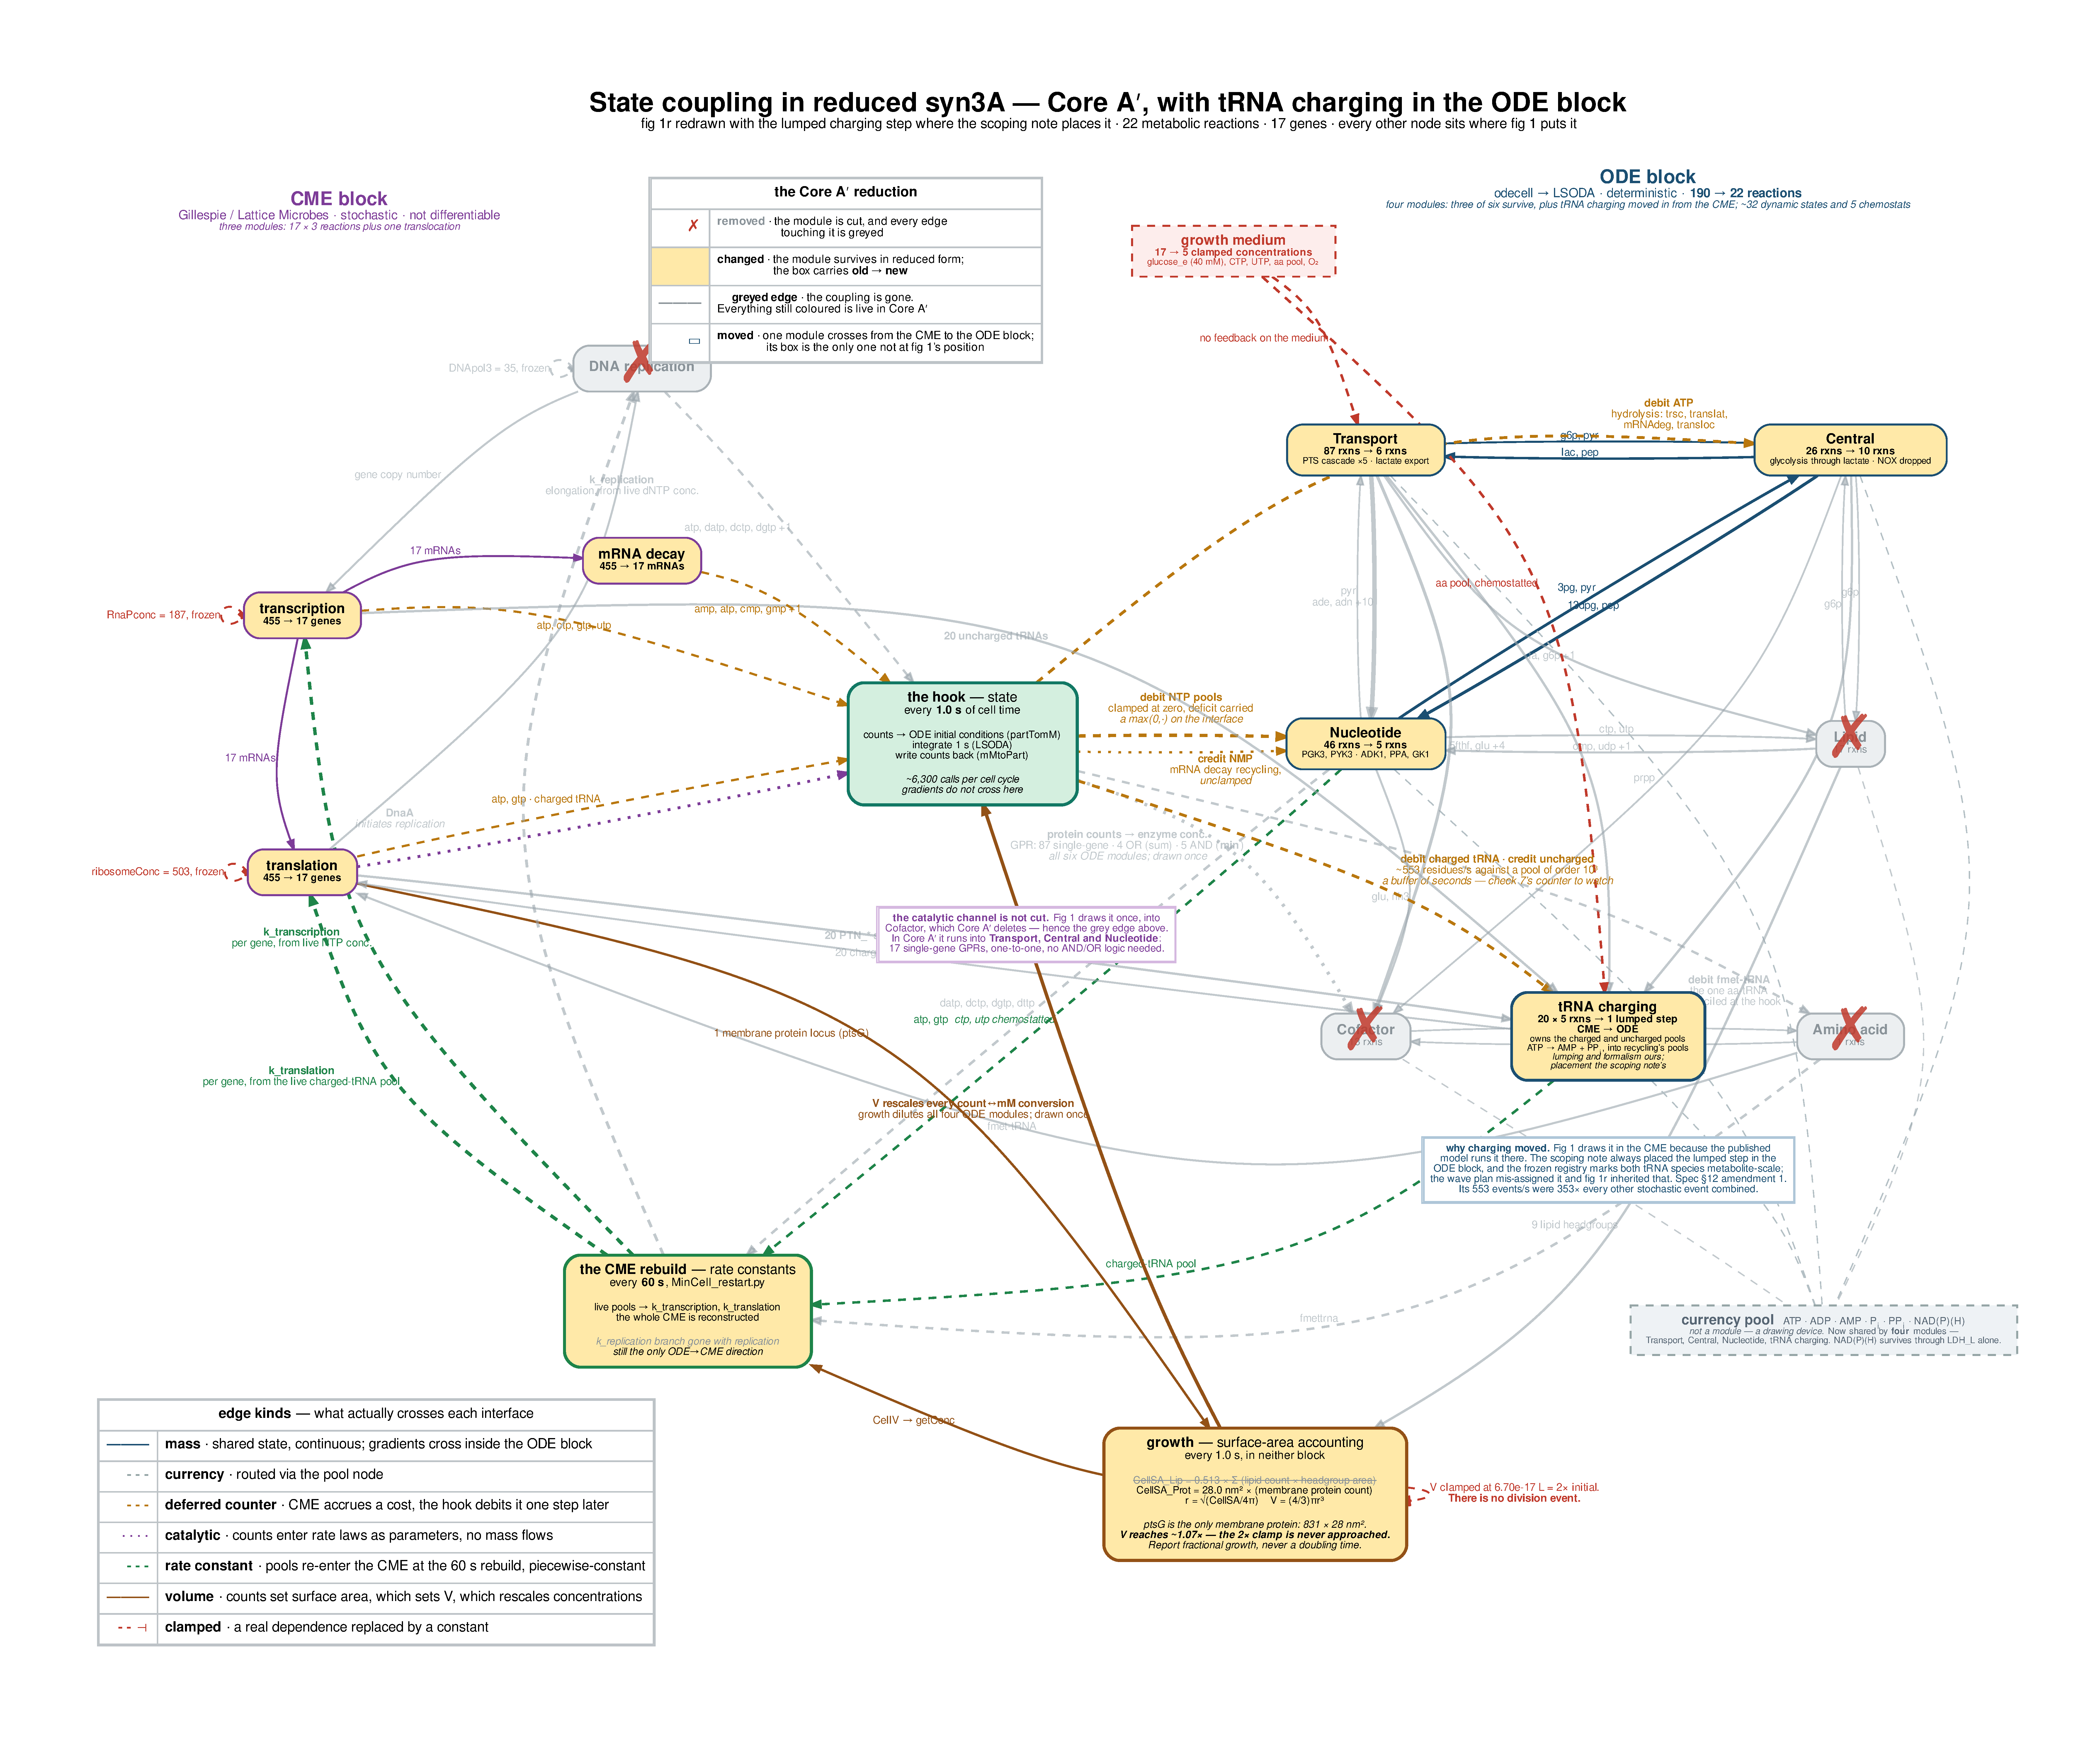
\includegraphics[width=0.85\textwidth]{fig1c_state_graph_corea.pdf}
\caption{\textbf{The reduced \syn{} model.} Metabolic modules (ODE) and
gene-expression modules (jump) and the edges between them.
\placeholder{Caption to be rewritten for the paper; the figure may need a cleaner
version for print.}}
\label{fig:model}
\end{figure*}

The model makes no claim about \syn{} itself. With most of the cell removed, it
cannot reproduce the doubling time, the metabolite levels or the proteome of the
real organism. The code refuses to report a doubling time, so that no result can
be compared with these quantities by mistake. The model's purpose is to give a
real ODE--stochastic boundary from a published whole-cell model, at a size where an
exact posterior is affordable.

\paragraph{M0, the reference system.} An exact posterior on the full reduced model
costs too much (\cref{sec:cost}). We therefore also use M0, the reduced model cut
to two genes over \pn{mzero.horizon}\,s. The two genes are GAPD, whose promoter is
the best determined, and ptsG, the membrane transporter. All metabolism stays. The
other enzyme counts are held at their measured copy numbers, and this hold is a
declared reduction. M0 has \pn{mzero.npar} free parameters: the two promoter
strengths, the transcript decay rate, the forward catalytic constants of enolase
(ENO) and aldolase (FBA), and the bulk assay noise $\sigb$.

\section{How information crosses the boundary}
\label{sec:seam}

Three problems are often treated as one.
\begin{itemize}
  \item \emph{Local inference:} what do a module's own data say about its own
  parameters?
  \item \emph{Uncertainty propagation:} given the uncertain output of one module,
  how uncertain is the next module?
  \item \emph{Cross-module inference:} do the data of one module inform the
  parameters of another, when the two share no parameter?
\end{itemize}
The third problem is the hard one, and it is the one this paper addresses.

\subsection{Three graphs}

A coupled model has three graphs, and they need not agree
(\cref{fig:graphs}). The \emph{coupling graph} says which module drives which
state. The \emph{likelihood graph} says which likelihood factors depend on which
parameters once the stochastic paths are integrated out. The \emph{information
graph} says which data streams move which parameters. In the reduced \syn{} model the
coupling graph is two-way, but the information graph is sparse and points mostly in
one direction.

\begin{figure}[t]
\centering
\placeholderfig{\columnwidth}{4.5cm}{Figure 3: the coupling, likelihood and
information graphs of the reduced model, side by side. To be drawn.}
\caption{\textbf{Three graphs of one model.} \placeholder{Caption.}}
\label{fig:graphs}
\end{figure}

Write $u$ for the trajectory at the interface: enzyme counts and drains in one
direction, pools in the other. For a pair of modules $A \to B$ with data $D_A$ and
$D_B$, the forward message is $p(u \mid D_A)$. The backward message is a likelihood
over the interface,
\begin{equation}
  \lambda_B(u) = \int p(D_B \mid \theta_B, u)\, p(\theta_B)\, \mathrm{d}\theta_B .
\end{equation}
The joint posterior over $u$ is proportional to $p(u \mid D_A)\,\lambda_B(u)$. A
\emph{statistical cut} drops $\lambda_B$ \citep{plummer2015cuts}. It changes the
target of inference, and data from $B$ can no longer inform $A$. A \emph{dynamical
reduction} instead removes a weak edge from the simulator and keeps full Bayesian
inference. For the question we ask, only the second kind keeps the information we
want: metabolite data that inform a gene-expression parameter.

\subsection{Information follows gain}

The strength of each coupling direction predicts where information flows
(\cref{tab:gain}). From gene expression to the pools the gain is of order one. The
pools turn over in seconds to minutes, and the drains from gene expression are a
large part of that turnover. From the pools back to the rate constants the gain is
small: an elasticity of \pn{gain.txlo}--\pn{gain.txhi} for transcription and
\pn{gain.tl} for translation. The gain is small because the published rate laws are
saturated. The half-saturation constant of RNA polymerase for its nucleotides is
\pn{gain.kd}\,mM, while ATP is near \pn{gain.atp}\,mM.

\begin{table}[t]
\caption{Gain and information in each direction across the boundary. Information is
the ratio of posterior to prior standard deviation from a linearised bound, at
200 cells and 10\% assay noise; the bracket is the ratio that noise alone gives.}
\label{tab:gain}
\centering
\small
\begin{tabular}{@{}p{0.3\columnwidth}p{0.25\columnwidth}p{0.33\columnwidth}@{}}
\toprule
Direction & Gain & Information \\
\midrule
Gene expression $\to$ pools & order one & ptsG from metabolites only: \pn{info.ptsg} (bracket \pn{info.ptsgbracket}) \\
Pools $\to$ rate constants & \pn{gain.txlo}--\pn{gain.txhi} (transcription), \pn{gain.tl} (translation) & ENO from transcripts only: \pn{info.enotx} \\
\bottomrule
\end{tabular}
\end{table}

So metabolite data can inform the ptsG promoter, a gene-expression parameter that
they never measure. Transcript data carry almost no information about the enolase
constant, a metabolic parameter. We report the second result as a measured null, not
as a failure. \placeholder{FBA under transcripts only is open; K2 at 1,000 cells
decides it (16b.5).}

\subsection{Why no parameter is shared}

The standard modular methods pass messages through shared parameters: cuts and
semi-modular inference \citep{plummer2015cuts,carmona2020semimodular}, and Markov
melding \citep{goudie2019joining}. In the reduced model no parameter is shared, so
these methods have nothing to pass while we condition on the stochastic path. The
exact sampler does what is left: it conditions on the path, and it updates the path
with all the data. In this sense the exact sampler is modular inference with nothing
dropped. When the paths are integrated out, a gene-expression parameter appears in
both the transcript factor and the metabolite factor. The approximate route uses
this structure.

\section{Results}
\label{sec:results}

All results use synthetic data. The data come from the full two-way model at known
parameter values, so the truth is known. The test of an inference method is then
calibration: over many datasets, a 90\% credible interval must contain the truth
about 90\% of the time \citep{talts2018validating}.

\subsection{The exact sampler is calibrated on M0}
\label{sec:exact}

\paragraph{Convergence.} We ran \pn{vsix.chains} chains of \pn{vsix.sweeps} sweeps on
one M0 dataset of \pn{mzero.cells} cells. The rank-normalised $\Rhat$
\citep{vehtari2021rank} is at most \pn{vsix.rhat}, and the bulk effective sample
size is at least \pn{vsix.ess} for every parameter. This reference run cost
\pn{vsix.cpuh} CPU-hours.

\paragraph{Calibration.} We drew \pn{vseven.R} parameter sets from the prior,
simulated one dataset from each, and fitted each dataset with one chain. For each
parameter we compared the empirical CDF of the ranks of the truth with a
simultaneous band \citep{sailynoja2022graphical}, at a joint level of 95\% over the
\pn{mzero.npar} parameters. All \pn{mzero.npar} parameters stay inside their bands
(\cref{fig:calibration}a). The largest deviation is \pn{vseven.maxdev}, for the
transcript decay rate, where the band allows \pn{vseven.band}. We also read coverage off the same ranks, for central credible intervals at five
levels from 50\% to 99\%. In \pn{vseven.cov} parameter--level pairs the coverage is
inside the binomial 95\% band. The one miss, the decay rate at 99\%, is where one or
two misses over 30 pairs are expected by chance.

\paragraph{A production-length chain matches the reference.} One chain of the
length we used in the calibration runs is not distinguishable from the reference on
any marginal (\cref{fig:calibration}b). The means differ by at most
\pn{ften.dmean} reference standard deviations, and the ratio of standard deviations
is between \pn{ften.sdlo} and \pn{ften.sdhi}. This chain cost \pn{ften.cpuh}
CPU-hours, about \pn{ften.speedup} times less than the reference.

\paragraph{Limits.} The calibration result holds for M0 only. In \pn{vseven.lowess}
of the \pn{vseven.R} replicates the smallest bulk effective sample size is below 100.
The production chain resolves the FBA constant from its matched null by a small
margin, \pn{ften.fbamargin} standard deviations.

\begin{figure*}[t]
\centering
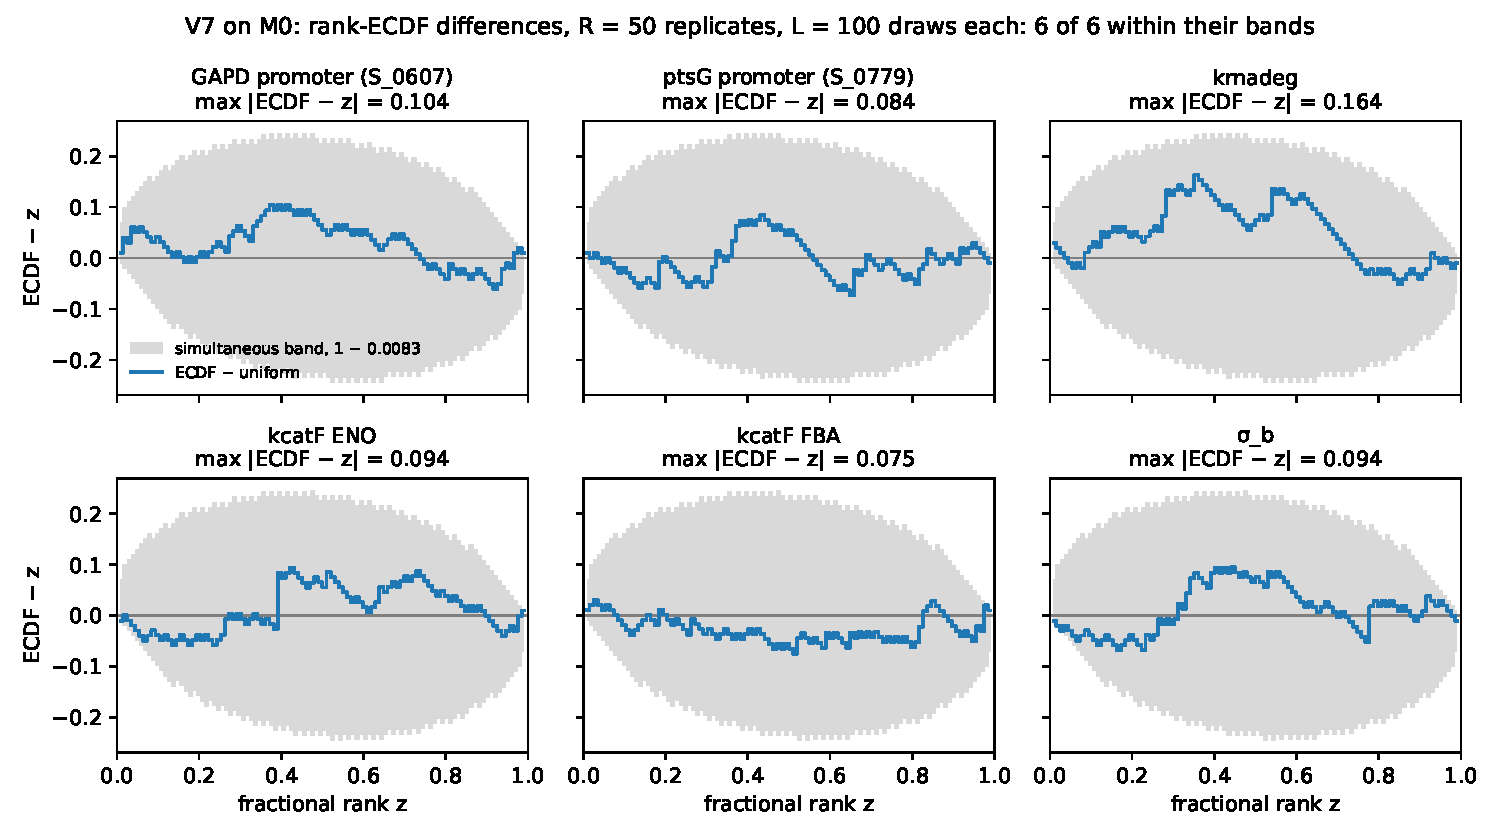
\includegraphics[width=0.48\textwidth]{f8_rank_ecdf.pdf}\hfill
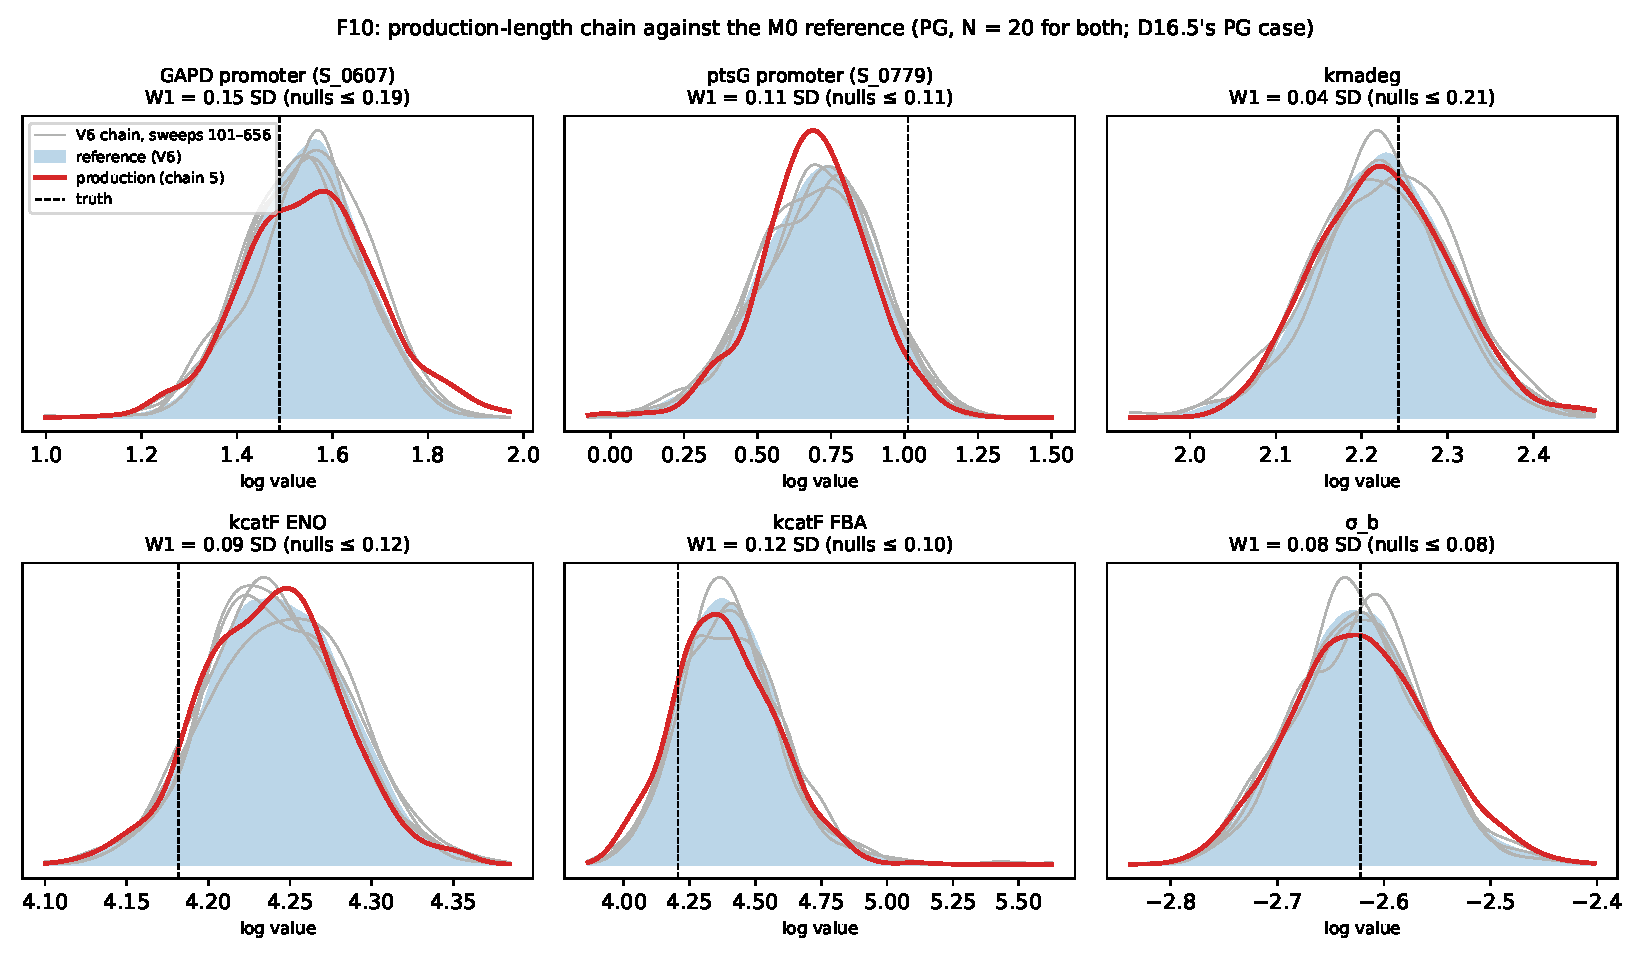
\includegraphics[width=0.48\textwidth]{f10_marginals.pdf}
\caption{\textbf{The exact sampler on M0.} (a) Rank-ECDF of the truth over
\pn{vseven.R} prior-drawn datasets, against simultaneous 95\% bands. (b) Marginal
posteriors from a production-length chain against the reference.
\placeholder{Restyle both panels to one figure with shared fonts; label panels.}}
\label{fig:calibration}
\end{figure*}

\subsection{The cost of the formalism swap is declared and measured}
\label{sec:jensen}

The mean-field swap replaces the stochastic gene expression with its mean. The
means of transcripts and proteins are exact, but metabolism is nonlinear. A
metabolism fed the mean drain differs from the mean over cells of metabolisms fed
their own drains. The difference is a Jensen gap.

\paragraph{The cause.} The gap is largest for GTP, where the mean field sits
\pn{jg.gtplo}--\pn{jg.gtphi}\% below the population mean. We traced it to
cell-to-cell variation in the drains. When every cell receives the mean field's
drains, the mean over cells equals the mean field to three significant figures. We
ruled out the enzyme counts, the per-cell feedback and the clip at zero as causes of
the GTP gap. A likely mechanism, which we have not tested, is that only saturable
enzymes regenerate GTP. Then cells that spend more GTP lose more of it than cells that
spend less gain back, and the population mean sits above GTP at the mean spend.

\paragraph{The correction.} We treat the gap as a declared reduction and correct it
with an offset $\delta$, the log difference between the mean of a reference
ensemble and the mean field at one reference parameter set. Our reference is the
most detailed composition we have, the exact hybrid, and not the truth about the
cell. We report the gap with a goodness check and with the parameter bias it
implies, and we do not use it as a stop.
\begin{itemize}
  \item Without $\delta$, the gap would move the transcript decay rate by
  \pn{jg.biaslo}--\pn{jg.biashi} posterior standard deviations.
  \item With $\delta$, the remaining bias is within about one standard deviation.
  \item The goodness check as first written fails a description known to be correct
  in about half of all cases: a correct description passes only
  \pn{jg.kgnulllo}--\pn{jg.kgnullhi}\% of the time. We therefore compare the check
  with its own null distribution. With $\delta$, the mean field falls inside the
  null's 95\% range at \pn{jg.deltain} targets, against \pn{jg.mfin} without
  $\delta$.
\end{itemize}

\paragraph{The mean-field model is the limit of the hybrid.} The hybrid exchanges
state every second. As this step shrinks, the hybrid's mean converges to the
one-ODE mean-field model. At the zero-step limit the two agree to
\pn{rii.maxdelta} in log concentration at all five test parameter sets. One
mean-field solve takes \pn{rii.mzero}\,s on M0 and \pn{rii.corealo}--\pn{rii.coreahi}\,s
on the full reduced model.

\placeholder{AV6 (B7) decides whether the remaining gap moves the posterior. Add one
sentence with the answer.}

\subsection{The approximate posterior agrees with the exact one on M0}
\label{sec:approx}

\placeholder{B7 / AV6, not run. Refit the \pn{vseven.R} V7 datasets with the
approximate route. Report: overlaid marginals and the ptsG--ENO contour against the
exact posterior; rank-ECDF of the approximate route; cost per posterior against
\pn{ften.cpuh} CPU-hours. Gate: M0 carries a metabolite $\to$ ptsG signal (linearised
ratio \pn{info.mzeroptsg} against a noise bracket of \pn{info.mzerobracket}; met).}

\begin{figure*}[t]
\centering
\placeholderfig{0.9\textwidth}{5cm}{Figure 5: approximate against exact on M0.
Overlaid marginals, the ptsG--ENO contour, rank-ECDF, and a cost bar. Not run (B7).}
\caption{\textbf{Approximate against exact.} \placeholder{Caption.}}
\label{fig:approx}
\end{figure*}

\subsection{Inference on the full reduced model}
\label{sec:fullscale}

\placeholder{B8 / AV7, not run; needs the cap reopened (O1). Calibration over
$\ge 200$ injections on the full reduced model. Posterior widths against the
linearised information bound for the six D11 targets. The F6 table: transcripts
only, metabolites only, both. Target from the bound: ptsG under metabolites only at
\pn{info.ptsg} of its prior SD (bracket \pn{info.ptsgbracket}); ENO at \pn{info.eno}
(bracket \pn{info.enobracket}).}

\begin{figure}[t]
\centering
\placeholderfig{\columnwidth}{5cm}{Figure 6 (F6): posterior/prior SD per target under
three data regimes, with the information bound drawn on. Not run (B8).}
\caption{\textbf{What each data stream informs.} \placeholder{Caption.}}
\label{fig:f6}
\end{figure}

\subsection{The uncertainty budget of a prediction}
\label{sec:budget}

\placeholder{Not built (outline §6). Draw the inferred parameters from the posterior
and all others from their priors; run the coupled model; split the variance of an
unobserved quantity (fractional growth, lactate export, or how often GTP empties)
into: inferred parameters, parameters left at their priors, and intrinsic noise.
Report the split with asserted prior widths halved and doubled. Target sentence:
``x\% of the uncertainty in this prediction comes from parameters that no
measurement supports.'' About 50 CPU-h on M0.}

\begin{figure}[t]
\centering
\placeholderfig{\columnwidth}{4.5cm}{Figure 7: the uncertainty budget of one
prediction. Not built.}
\caption{\textbf{Where the uncertainty of a prediction comes from.}
\placeholder{Caption.}}
\label{fig:budget}
\end{figure}

\subsection{Cost}
\label{sec:cost}

\Cref{tab:cost} gives the cost of one posterior by each route. An exact posterior on
the full reduced model is projected at about \pn{cost.fullscale} CPU-hours, above
our bound of \pn{cost.kone} CPU-hours per posterior. Exact inference therefore
stops at M0. The cost is the number of simulations, not the time of one. One cycle
of the full reduced model takes \pn{model.cyclewall}\,s, and a fast
implementation of the full \syn{} model is the subject of a companion paper
\citep{kimpson2026whole}.

\begin{table}[t]
\caption{CPU-hours per posterior.}
\label{tab:cost}
\centering
\small
\begin{tabular}{@{}lcc@{}}
\toprule
Route & M0 & Reduced model \\
\midrule
Exact, reference & \pn{vsix.cpuh} & --- \\
Exact, production & \pn{ften.cpuh} & $\sim$\pn{cost.fullscale} (projected) \\
Approximate & \placeholder{B7} & \placeholder{B8} \\
\bottomrule
\end{tabular}
\end{table}

\section{Discussion}
\label{sec:discussion}

\placeholder{Opening paragraph: restate the main result once B7 and B8 are in.}

\paragraph{What scales and what does not.} Exact inference across the boundary works,
and it is calibrated, but it stops at M0. The cost of an exact posterior grows with
the number of genes and the length of the record, and the full reduced model is
already above our budget. The approximate route removes the stochastic paths from
the sampler. Two quantities limit it. The first is the Jensen gap, which we declare
and correct (\cref{sec:jensen}). The second is $R$, the variance of the bulk
log-likelihood over the paths that the transcripts allow. $R$ is about
\pn{info.Rmzero} on M0 and \pn{info.Rcorea} on the full reduced model at 10\% assay
noise. So the metabolites constrain the paths together, and a single draw of paths
per parameter value is not enough. The Gaussian bulk factor handles this regime.
\placeholder{Confirm once B7 reports.}

\paragraph{The observation model sets the interface.} The three graphs of
\cref{sec:seam} give a general rule. Single-cell data inform the parameters of their
own module. Information between modules travels on bulk observables, and it follows
the gain of the coupling. A modeller can compute the gains before any inference, and
in this work the gains predicted the information in each direction before any
posterior existed.

\paragraph{Reductions as approximations to inference.} A dynamical reduction changes
the simulator and keeps full Bayesian inference. A statistical cut keeps the
simulator and changes the target. We prefer the first, because its cost can be
measured against a more detailed composition. The formalism swap is such a reduction.
We do not claim that the more detailed composition is the truth about the cell. We
claim that each choice of description is declared, and that its cost is measured.

\subsection{Limitations}

\begin{itemize}
  \item \emph{Synthetic data only.} The data come from the model itself. Real
  assays need observation models for unknown cell numbers in bulk metabolomics and
  for capture efficiency in single-cell RNA counts.
  \item \emph{One organism, one reduction.} We demonstrate the framework on one
  reduced model. \placeholder{O3: build the generic registry, or narrow the
  framework claim to ``demonstrated on one organism''.}
  \item \emph{Asserted priors.} Many priors have no width in their source, so we set
  the width. The uncertainty budget (\cref{sec:budget}) reports how much this choice
  matters. \placeholder{Once built.}
  \item \emph{Exact calibration at small scale only.} Coverage of the exact sampler
  at the full reduced model is out of reach at about \pn{cost.fullscale} CPU-hours per
  posterior.
  \item \emph{Weak reverse coupling.} The approximate route relies on the small
  elasticities of the rebuild (\pn{gain.txlo}--\pn{gain.tl}). A perturbation that
  drains the nucleotide pools toward the half-saturation constant would remove this
  basis.
\end{itemize}

\subsection{Future work}

\placeholder{One short paragraph, in this order: (1) the method's own limits:
condition the bulk factor on the observed transcripts; path sampling only for pools
near the one-particle floor; strong-feedback regimes. (2) The full well-stirred
\syn{} model through the syn3a-ensemble port, then real data. (3) Comparing model
structure and formalisms, which the swap makes possible, by predictive scores rather
than Bayes factors. (4) Goal-directed inference and experimental design: which parts
of a coupled simulator must be kept, and which latent variables inferred, to keep
the information a prediction needs?}

\section*{Software and data availability}
\label{sec:availability}

\IC{} is open source at \url{https://github.com/MACSYS-CoE/InferCell}, with
documentation at \url{https://macsys-coe.github.io/InferCell/}. The test suite has
\pn{fw.tests} assertions. \placeholder{Release tag and archived DOI (Zenodo) for the
version used in this paper.} \placeholder{Archive of the posterior draws and result
files, with the scripts and commits that produced each number.}

\section*{Acknowledgements}
\placeholder{Funding, computing resources (OzSTAR), collaborators.}


\bibliography{references}
\bibliographystyle{icml2026}

\newpage
\appendix
\onecolumn
\section{Methods}
\label{sec:methods}

\placeholder{Venue decides the form: STAR Methods (Cell Systems) or a Methods section
after the Discussion (PLOS CB). Content is the same.}

\subsection{The hybrid driver}
\label{sec:driver}

The driver keeps two blocks with separate state: metabolite pools in mM as floating
point values, and molecule counts as integers. One handshake step does the
following, in order:
\begin{enumerate}
  \item update growth and cell geometry from the membrane protein counts;
  \item write the protein counts into the metabolic rate laws (catalytic edges);
  \item step the ODE block by 1\,s (Rodas5P, absolute tolerance $10^{-10}$, relative
  tolerance $10^{-8}$);
  \item debit the pools by the costs of the stochastic events of the previous step
  (deferred-cost edges), clipped at zero as in the published model;
  \item every 60\,s, rebuild the stochastic rate constants from the pools;
  \item step the jump block by 1\,s with Gillespie's direct method
  \citep{gillespie1977exact}.
\end{enumerate}
On the jump clock the rebuilt constants therefore take effect at $60m - 1$\,s. Pools
are written back as molecule counts under a declared rounding policy. A recorded path
can be replayed: the replay applies the recorded firings instead of drawing new ones,
and it returns the log density of the path and its sufficient statistics (event
counts and exposures).

\subsection{Observation model}
\label{sec:obs}

Each synthetic dataset has $C$ cells (\pn{mzero.cells} on M0), observed every 60\,s.
\begin{itemize}
  \item \textbf{Transcripts:} the exact count of each gene's transcripts in each cell
  at each save.
  \item \textbf{Bulk metabolites:} one measurement per pool per save of the mean over
  the $C$ cells, $\bar{x}$, with lognormal noise: $\log z \sim
  \mathcal{N}(\log \bar{x}, \sigb^2)$. The assay noise $\sigb$ is a free parameter.
\end{itemize}
We use bulk metabolites because a per-cell metabolite panel cannot be measured.
\placeholder{State the panel (M0\_PANEL) and the prior on $\sigb$.}

\subsection{The exact sampler}
\label{sec:sampler}

The sampler is a three-block Gibbs scan with the stochastic path as a latent variable.
\begin{enumerate}
  \item \textbf{Paths.} Conditional sequential Monte Carlo over 60\,s windows
  \citep{andrieu2010particle}, with particle Gibbs at $N = 20$ particles. Each
  particle is a snapshot of the driver. Transcripts are proposed as exact
  endpoint-conditioned birth--death bridges \citep{hobolth2009simulation}, so every
  proposal agrees with the observed transcript counts. The other reactions are then
  simulated given the transcripts. The weight is the bulk metabolite likelihood
  times each gene's transition probability. Cells are updated in turn, because the
  bulk likelihood couples them.
  \item \textbf{Metabolic constants and $\sigb$.} A univariate slice step on each log
  parameter, given the paths. Reverse constants follow from the forward ones and the
  equilibrium constants.
  \item \textbf{Gene-expression constants.} Given the path, each promoter strength
  and the decay rate have an exact one-dimensional conditional of the form
  $n u - e^{u} A + \log p(u)$, where $n$ is the event count and $A$ the exposure. We
  sample it by a slice step.
\end{enumerate}
The sampler is written directly, not in a probabilistic programming language. The
path update needs ancestor sampling and exact snapshots of the driver, and a general
framework could not provide them without sharing solver state between particles.
Runs can be checkpointed and resumed bit for bit, and the threaded sweep is bit for
bit equal to the serial one.

\subsection{The transcript factor}
\label{sec:txfactor}

When the paths are integrated out, each gene's transcripts form a birth--death chain
with a piecewise-constant birth rate, observed exactly every 60\,s. The likelihood of
one cell's record is a product of transition probabilities. We compute them by
uniformisation with tridiagonal products, truncated where the remaining mass is below
$10^{-12}$. The cap on the count is fixed per dataset, and the number of terms comes
from the primal value, so the factor is differentiable in the rates.

\subsection{The mean-field route}
\label{sec:meanfield}

The swap replaces the three jump modules with one mean-field module. Its equations
are generated from the jump modules' own propensities and update rules. The composed
model is one ODE problem. Four edges change form, and each change is a declared
reduction:
\begin{itemize}
  \item catalytic edges read the mean protein counts;
  \item drains are continuous and not clipped, and the solve stops if a pool becomes
  negative;
  \item the rebuild is a discrete callback at $60m - 1$\,s and at $t = 0$;
  \item growth is continuous.
\end{itemize}
The bulk factor is $\mathcal{N}\!\left(\log z;\ \log \max(\bar{x}_{\mathrm{MF}}(\theta), 1)
+ \delta,\ \sigb^2 I + S\right)$, with $\delta$ and $S$ from an ensemble of the exact
hybrid at a reference parameter value, and the floor of one molecule.
\placeholder{B5: state how S is estimated (delta method over 800 cells) and the
sampler settings once built.}

\subsection{Simulation-based calibration}
\label{sec:sbc}

For each of $R = \pn{vseven.R}$ replicates we drew a parameter set from the prior,
simulated a dataset, and ran one chain of 656 sweeps from a prior draw. We dropped
100 sweeps and thinned the rest to $L = 100$ draws. The rank of the truth among the
draws is uniform if the sampler is calibrated \citep{talts2018validating}. We tested
each parameter's rank-ECDF against a simultaneous band at $1 - 0.05/6$
\citep{sailynoja2022graphical}, so the test as a whole is at the 95\% level. The pass
rule was fixed before any rank was computed.

\subsection{Compute}
\label{sec:compute}

All runs used the OzSTAR cluster. \placeholder{Hardware, total CPU-hours, and a table
of every job behind each number, from the result files.}


\end{document}
